\begin{solution}
The answer is negative.\\[0.2cm]
Assume that we color the first and fourth rows of the table in gray as shown below:

\begin{center}
	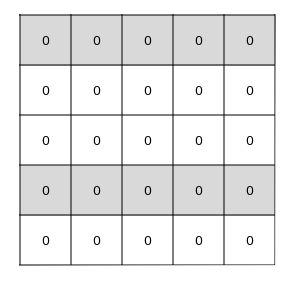
\includegraphics[width=10cm]{63/figs/63_sol2.png}
\end{center}

Notice that any $2 \times 2$ or $3 \times 3$ subtable contains an even number of white cells. Therefore, each move will toggle an even number of white cells, and the parity of the sum of the numbers of white squares will always remain even. Thus we can never turn the table into a configuration in which the number of 1s in the white cells is odd.
\end{solution}
